\begin{picture}(0,0)%
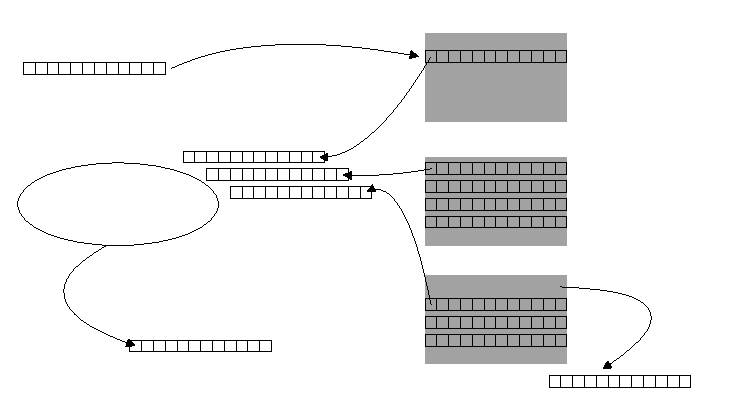
\includegraphics{figs/induced_operation.fig.eps}%
\end{picture}%
\setlength{\unitlength}{4144sp}%
%
\begingroup\makeatletter\ifx\SetFigFontNFSS\undefined%
\gdef\SetFigFontNFSS#1#2#3#4#5{%
  \reset@font\fontsize{#1}{#2pt}%
  \fontfamily{#3}\fontseries{#4}\fontshape{#5}%
  \selectfont}%
\fi\endgroup%
\begin{picture}(5444,2829)(218,-2236)
\put(271,299){\makebox(0,0)[lb]{\smash{{\SetFigFontNFSS{10}{12.0}{\familydefault}{\mddefault}{\updefault}{\color[rgb]{0,0,0}$r.name = C_1$}%
}}}}
\put(271,434){\makebox(0,0)[lb]{\smash{{\SetFigFontNFSS{10}{12.0}{\familydefault}{\mddefault}{\updefault}{\color[rgb]{0,0,0}$r.row = n$}%
}}}}
\put(1081,-1681){\makebox(0,0)[lb]{\smash{{\SetFigFontNFSS{10}{12.0}{\familydefault}{\mddefault}{\updefault}{\color[rgb]{0,0,0}$out.row = n$}%
}}}}
\put(1081,-1816){\makebox(0,0)[lb]{\smash{{\SetFigFontNFSS{10}{12.0}{\familydefault}{\mddefault}{\updefault}{\color[rgb]{0,0,0}$out.name = f()$}%
}}}}
\put(4456,254){\makebox(0,0)[lb]{\smash{{\SetFigFontNFSS{10}{12.0}{\familydefault}{\mddefault}{\updefault}{\color[rgb]{0,0,0}n}%
}}}}
\put(4456,-601){\makebox(0,0)[lb]{\smash{{\SetFigFontNFSS{10}{12.0}{\familydefault}{\mddefault}{\updefault}{\color[rgb]{0,0,0}n}%
}}}}
\put(4456,-736){\makebox(0,0)[lb]{\smash{{\SetFigFontNFSS{10}{12.0}{\familydefault}{\mddefault}{\updefault}{\color[rgb]{0,0,0}n+1}%
}}}}
\put(4456,-871){\makebox(0,0)[lb]{\smash{{\SetFigFontNFSS{10}{12.0}{\familydefault}{\mddefault}{\updefault}{\color[rgb]{0,0,0}n+2}%
}}}}
\put(4456,-1006){\makebox(0,0)[lb]{\smash{{\SetFigFontNFSS{10}{12.0}{\familydefault}{\mddefault}{\updefault}{\color[rgb]{0,0,0}n+3}%
}}}}
\put(4456,-1636){\makebox(0,0)[lb]{\smash{{\SetFigFontNFSS{10}{12.0}{\familydefault}{\mddefault}{\updefault}{\color[rgb]{0,0,0}n}%
}}}}
\put(4456,-1771){\makebox(0,0)[lb]{\smash{{\SetFigFontNFSS{10}{12.0}{\familydefault}{\mddefault}{\updefault}{\color[rgb]{0,0,0}n+1}%
}}}}
\put(4456,-1906){\makebox(0,0)[lb]{\smash{{\SetFigFontNFSS{10}{12.0}{\familydefault}{\mddefault}{\updefault}{\color[rgb]{0,0,0}n+2}%
}}}}
\put(3286,434){\makebox(0,0)[lb]{\smash{{\SetFigFontNFSS{12}{14.4}{\familydefault}{\mddefault}{\updefault}{\color[rgb]{0,0,0}$C_1$}%
}}}}
\put(3331,-1321){\makebox(0,0)[lb]{\smash{{\SetFigFontNFSS{12}{14.4}{\familydefault}{\mddefault}{\updefault}{\color[rgb]{0,0,0}$C_3$}%
}}}}
\put(3331,-421){\makebox(0,0)[lb]{\smash{{\SetFigFontNFSS{12}{14.4}{\familydefault}{\mddefault}{\updefault}{\color[rgb]{0,0,0}$C_2$}%
}}}}
\put(5401,-2221){\makebox(0,0)[lb]{\smash{{\SetFigFontNFSS{10}{12.0}{\familydefault}{\mddefault}{\updefault}{\color[rgb]{0,0,0}n-1}%
}}}}
\put(4861,-1501){\makebox(0,0)[lb]{\smash{{\SetFigFontNFSS{10}{12.0}{\familydefault}{\mddefault}{\updefault}{\color[rgb]{0,0,0}Delete}%
}}}}
\put(271,-1231){\makebox(0,0)[lb]{\smash{{\SetFigFontNFSS{10}{12.0}{\familydefault}{\mddefault}{\updefault}{\color[rgb]{0,0,0}Eval}%
}}}}
\put(361,-871){\makebox(0,0)[lb]{\smash{{\SetFigFontNFSS{10}{12.0}{\familydefault}{\mddefault}{\updefault}{\color[rgb]{0,0,0}$f(C_1,C_2,C_3)$}%
}}}}
\end{picture}%
